\part*{Guide}\addcontentsline{toc}{part}{Guide}
%----------------------------------------------------------------------------
\chapter{Getting started}\label{app:start}
%----------------------------------------------------------------------------
This guide is the starter pack of the FTSRG advisors, Martin Farkas (\href{https://github.com/BlackLight54}{\texttt{BlackLight54}} on GitHub) and Imre Kocsis (\href{https://github.com/imrekocsis}{\texttt{imrekocsis}}): what to do before you write, how a TDK paper comes together, how we work together, and the tools we recommend.
It comes at the end of the paper template, after the appendices. Nothing has to be deleted before you submit: \texttt{reviewer.tex} builds the paper without the guide and without any note (\cref{app:latex:todo}), and that PDF is the one you upload.

The template uses three kinds of notes. \todo[inline]{An orange note is for you: what a part of the paper must contain.}
\advisortodo{A blue note is for us: a draft we still have to confirm, or a link we still have to add.}
\atodo[inline]{A green note, marked A, is our review comment on your paper. Resolve it, then delete it.}

Work through the steps below in order in your first week. Each says who does it.

%----------------------------------------------------------------------------
\section{Share your identifiers}\label{app:start:ids}
\emph{You.} Send us your Neptun code, your GitHub username, and your \texttt{@edu.bme.hu} email address, in a Teams chat message or an e-mail to both of us; our faculty addresses are on the \href{https://ftsrg.mit.bme.hu/en/about/}{research group's page}. We use them to add you to the Overleaf project, the repositories and the Zotero group.

%----------------------------------------------------------------------------
\section{Accounts and access}\label{app:start:access}
\paragraph{Overleaf project.} \emph{We} create an Overleaf project for your semester's work from this template, so that you get the features of our Overleaf Pro subscription. Ask us for it. The template is the current BME template, modified to the TDK form requirements (\cref{app:tdk:form}); check that it still matches the current call.

\paragraph{Repositories.} Your work lives in three GitHub repositories, cloned as one (\cref{app:code:github}):
\begin{itemize}
  \item \textbf{Notes repository}, the top level: notes, drawings, consultation summaries and presentations, and a README that links the pieces. \emph{You} create it, and it includes the other two as Git submodules.
  \item \textbf{\texttt{paper/}}, the paper repository: \emph{we} connect the Overleaf project to a new GitHub repository with Overleaf's GitHub integration. Only the owner of the Overleaf project can use this Pro feature, and only with a fresh repository, so we create it and add you. Overleaf and GitHub stay in sync through the GitHub dialog in Overleaf's menu.
  \item \textbf{\texttt{code/}}, the code repository: \emph{you} create it from our template, with everything Zenodo needs to archive it (\cref{app:zenodo}).
\end{itemize}
Add both of us to all three, add \texttt{paper/} and \texttt{code/} to the notes repository as submodules, and clone it with \texttt{git clone --recurse-submodules}. One clone then holds everything: you can compile the paper locally, use every GitHub feature, and work with agent-based AI tools across notes, paper and code (\cref{app:code:ai}).

\paragraph{Zotero group.} \emph{We} add you to our Zotero group, \href{https://www.zotero.org/groups/6715800/ftsrg_blockchain_lab}{ftsrg\_blockchain\_lab}, where we collect the literature of our topics. \emph{You} install \href{https://www.zotero.org/}{Zotero} with its browser connector and save every source you read into the group library.

The paper gets the library through Overleaf's Zotero integration, another feature of our Pro subscription. Link your Zotero account in Overleaf's account settings, in the \emph{Reference Managers} section. Then, in the project, delete the placeholder \texttt{bib/zotero.bib}, choose \emph{New file}, then \emph{From Zotero}, pick the group library, and name the file \texttt{bib/zotero.bib}. The \emph{Refresh} button on the file brings in new sources. A refresh overwrites the file, so keep hand-written entries, such as the Zenodo artifact and AI citations, in \texttt{bib/references.bib}; the paper reads both. Working locally without Overleaf, the Better BibTeX plugin of Zotero can export the group to the same file.

\paragraph{GitHub Student Developer Pack.} Apply for the free \href{https://education.github.com/pack}{GitHub Student Developer Pack} with your \texttt{@edu.bme.hu} address; it includes GitHub Pro and GitHub Copilot.

%----------------------------------------------------------------------------
\section{Calendar}\label{app:start:calendar}
\paragraph{Neptun timetable.} \emph{You.} In Neptun's calendar, choose \emph{Naptár kezelése}, then \emph{Feliratkozás link másolása} (\cref{fig:neptun-export}): this exports your timetable \emph{as a link}, so it stays up to date. Add the link to the calendar you use; in Google Calendar, it is \emph{Settings}, \emph{Add calendar}, \emph{From URL} (\cref{fig:google-calendar-url}).
\begin{figure}[!ht]
  \centering
  \begin{subfigure}[b]{0.55\linewidth}
    \centering
    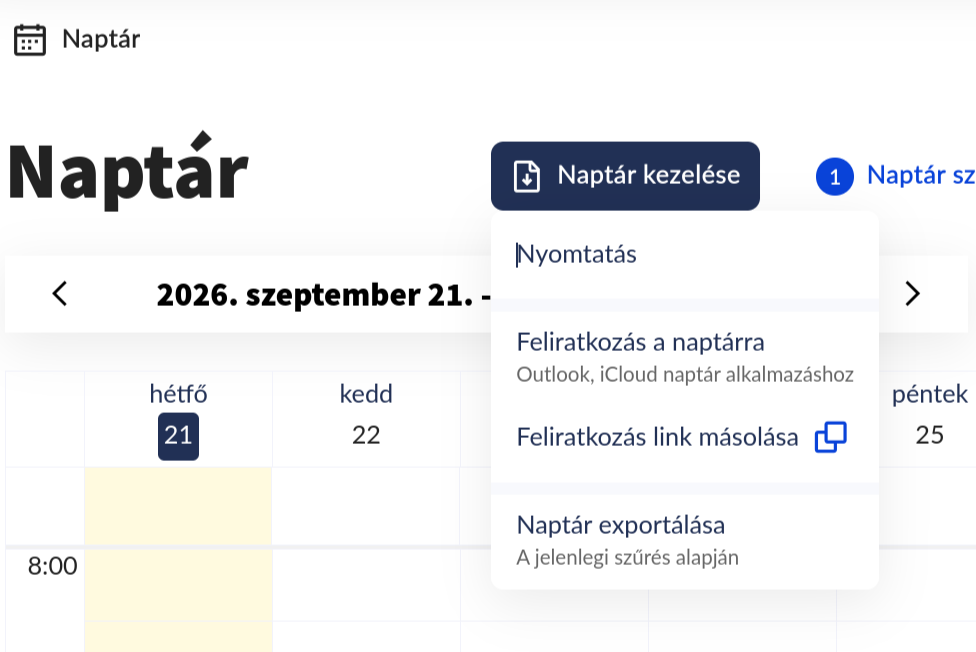
\includegraphics[width=\linewidth]{figures/neptun-calendar-export}
    \caption{Neptun: copy the subscription link.}\label{fig:neptun-export}
  \end{subfigure}\hfill
  \begin{subfigure}[b]{0.3\linewidth}
    \centering
    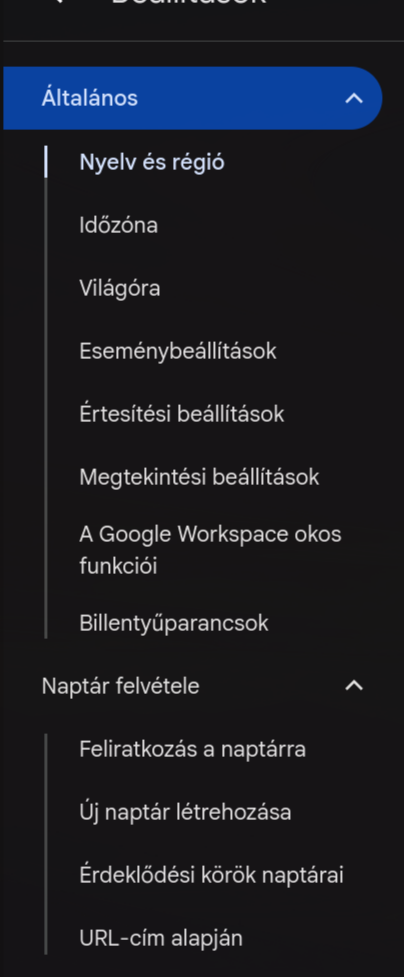
\includegraphics[width=0.75\linewidth]{figures/google-calendar-add-by-url}
    \caption{Google Calendar: add it from the URL.}\label{fig:google-calendar-url}
  \end{subfigure}
  \caption{Exporting the Neptun timetable to a calendar as a link.}\label{fig:neptun-calendar}
\end{figure}

\paragraph{Share it with your advisors.} In the Teams calendar, add your advisors' calendars: \emph{Add calendar}, type their name, add them. Ask them to give you permission to see their calendar, and share yours with them, so we can find a weekly slot (\cref{app:consult}).

\paragraph{Keeping calendars in sync.} We recommend \href{https://reclaim.ai/}{Reclaim.ai} to manage your calendar. You will likely run into permission issues with the university account; if so, \href{https://www.outlookgooglecalendarsync.com/}{Outlook Google Calendar Sync} is a workaround.

%----------------------------------------------------------------------------
\section{Development environment}\label{app:start:env}
\paragraph{Operating system.} Use Linux on bare metal if you can. We recommend \href{https://omarchy.org/}{Omarchy}, an easy-to-use distribution set up for development; ask Martin for his setup. Ubuntu and Pop!\_OS are good options too. Omarchy has a built-in Windows virtual machine; dual boot if you occasionally need Windows on bare metal. Use the Windows Subsystem for Linux (WSL) only as a last resort, if you really have to use Windows every day for a pressing reason, such as video editing.

\paragraph{Editor.} We use \href{https://code.visualstudio.com/}{Visual Studio Code}. Useful extensions: LaTeX Workshop to build the paper locally, Remote - SSH to work on the VM, GitHub Pull Requests, the Claude Code and Codex extensions, and the language extensions of your code.

\paragraph{Virtual machine.} We can give you a virtual machine with 8 cores and 16\,GB of memory in the \href{https://cloud.bme.hu/}{BME cloud}, most likely in its \href{https://fured.cloud.bme.hu/}{Füred} environment. Ask us for it directly, in the same message as your identifiers: say that you need a VM set up in the BME cloud, and we request it for you. Use it to host your editor and repositories remotely, and to run AI agents that keep working while your laptop is closed. Reach it through SSH, RDP, VS Code Remote, or Tailscale, or run Claude Code, Codex, T3 Code or GitKraken Kepler on it directly.

\paragraph{Workspace layout.} Keep one clone of the notes repository, with its \texttt{paper/} and \texttt{code/} submodules (\cref{app:code:github}), on your machine or on the VM. Open it in one VS Code window with the \LaTeX{} build and an AI agent working in the same folder, so that code, paper and notes are edited, versioned and searched together. The point is that an agent that can see the paper while it edits the code, and the consultation notes while it edits either, makes far fewer mistakes than one that sees a single repository. Commit in each submodule separately, and commit the submodule pointers in the notes repository after a consultation, so that the state you discussed is the state we can check out.

\paragraph{Do not overdo it.} Do not spend too much time on your environment setup. We learned this the hard way.
